\section{数据处理与问题分析}
\subsection{数据门禁与统一口径}
全年负荷、光伏和波动电价数据均为$365\times144$，每日四次光伏预报形成1,460个唯一“日期--发布时刻”键。检查结果为数值缺失0、负值0、重复日期0。负荷范围为1,995.7176--7,978.8849 kW，光伏为0--10,216.2000 kW，波动电价为0.0076--1.7936元/kWh。夜间光伏零值具有物理意义，予以保留；光伏预报表的日期结构空白采用向下填充恢复。

功率进入能量平衡前按
\begin{equation}\Delta t=\frac16\ \mathrm{h},\qquad E_{d,t}=P_{d,t}\Delta t\label{eq:conversion}\end{equation}
转换为时段电量。原始144点按官方结果模板的行序一一对应，另以整体平移$\pm10$分钟检验标签歧义。决策日$d$的模型只能读取$d$以前的实测数据及决策时已经发布的预报，事后实测轨迹仅用于结算，避免未来信息泄漏。数据流程见图~\ref{fig:pipeline}。
\begin{figure}[H]\centering
\includegraphics[width=\textwidth]{../figures/fig_pipeline.pdf}
\caption{数据门禁、信息集切分与无泄漏建模流程}\label{fig:pipeline}\end{figure}
\subsection{四问递进关系}
问题一提供确定性线性规划基座；问题二加入预测与紧急购电；问题三只对尚未执行时段滚动重算，并把“不调整”保留为可行基线；问题四只改变电价过程和其可见信息，不改变能量平衡。这样可将性能差异归因于新增信息或价格机制，而不是模型口径变化。
\begin{figure}[H]\centering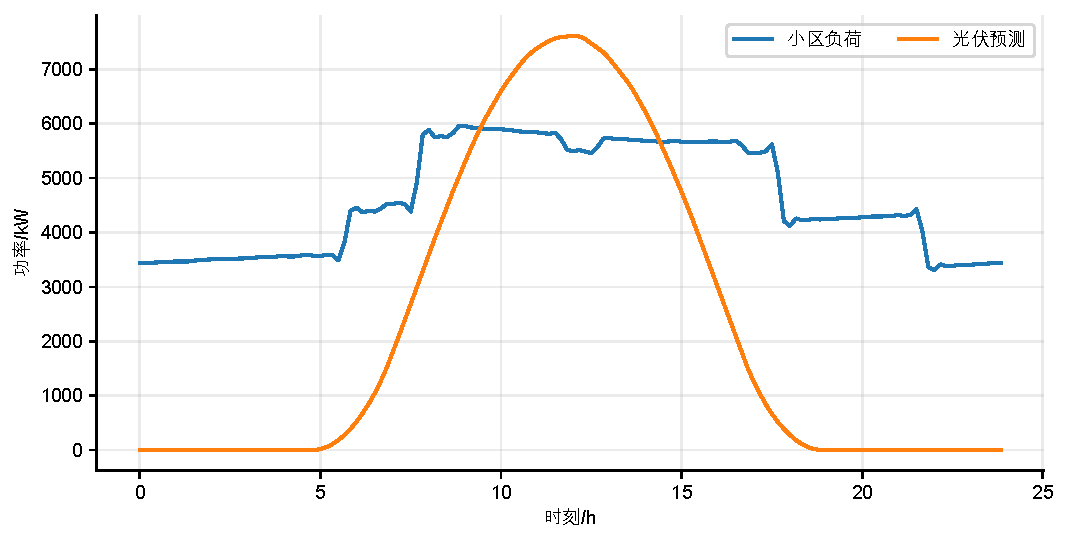
\includegraphics[width=0.92\textwidth]{../figures/fig01_input_profiles.pdf}
\caption{附件一负荷与光伏功率的日内变化}\label{fig:input}\end{figure}
